\documentclass{IOS-Book-Article}
\usepackage[utf8]{inputenc}
\usepackage{graphicx}
\usepackage{framed}
\usepackage[normalem]{ulem}

\def\hb{\hbox to 11.5 cm{}}

\newcommand{\sembrack}[1]{[\![#1]\!]}
\newcommand{\subex}[2]{#1_{#2}}
\newcommand{\commentOut}[1]{}
\newcommand{\eop}[1]{\mbox{\textsl{#1}}}
\newcommand{\ttop}[1]{\mbox{\texttt{#1}}}

\newcommand{\bequ}{\begin{quote}}
\newcommand{\enqu}{\end{quote}}
\newcommand{\bece}{\begin{center}}
\newcommand{\ence}{\end{center}}
\newcommand{\todoj}[1]{{\color{red}\textbf{[J: #1]}}}
\newcommand{\todoi}[1]{{\color{magenta}\textbf{[I: #1]}}}

\newenvironment{compactitem}{\begin{itemize}}{\end{itemize}}

\begin{document}

\pagestyle{headings}
\def\thepage{}
\begin{frontmatter}              % The preamble begins here.

\title{An End-to-End Pipeline from Law Text to Logical Formulas}

\markboth{}{October 2022 - Final Version\hb}

\author[A]{Aarne Ranta}
\author[B,C]{Inari Listenmaa}
\author[C]{Jerrold Soh}
\author[C]{Meng Weng Wong}

\address[A]{
   Department of Computer Science and Engineering,
   Chalmers University of Technology and University of Gothenburg,
   aarne.ranta@cse.gu.se
   }
 \address[B]{Digital Grammars AB}
 \address[C]{Centre for Computational Law, Singapore Management University}

\begin{abstract}
 This paper develops a pipeline for converting natural English law texts into logical formulas via a series of structural representations. The goal is to study how law-to-logic translation can be achieved with a sequence of well-defined steps. The texts are first parsed using a formal grammar derived from light-weight text annotations designed to minimise the need for manual grammar construction. An intermediate representation, called assembly logic, is then used for logical interpretation and supports translations to different back-end logics and visualisations. The approach, while rule-based and explainable, is also robust: it can deliver useful results from day one, but allows subsequent refinements and variations. While some work is needed to extend the method to new laws, the software presented here reduces the marginal effort necessary. As a case study, we demonstrate our approach on one part of Singapore’s Personal Data Protection Act. Our code is available open-source.
\end{abstract}

\begin{keyword}
legal formalisms, legal text parsing, Grammatical Framework, context-free grammars, methodology
\end{keyword}
\end{frontmatter}
\markboth{October 2022 - Final Version\hb}{October 2022 - Final Version\hb}

%\maketitle
\section{Introduction}

Expressing laws computably is a classic objective of AI \& Law \cite{mccarty_reflections_1977, sergot_british_1986} and a crucial pre-requisite to automating downstream tasks such as
compliance checking \cite{palmirani_modelling_2018, hickey_gdpr_2021},
policy support \cite{svensson_expertisze_1992, haan_tracs_1992},
%%%information retrieval \cite{bing_designing_1987},
%%%argumentative reasoning \cite{mochales_study_2008},
legislative simulation \cite{bench-capon_logic_1987, bench-capon_support_1992},
and formal verification \cite{haan_tracs_1992}.
But faithfully translating law to logic is challenging, often requiring expertise in both legal and formal methods. This ``natural language barrier'' \cite{mccarty_deep_2007} poses a significant ``knowledge bottleneck'' \cite{nazarenko_pragmatic_2021} to computational law systems.
Numerous strategies have been devised for bridging the gap.
These include
domain-specific ontologies \cite{palmirani_legal_2018},
taxonomies \cite{hulstijn_taxonomy_2020},
vocabularies \cite{hickey_gdpr_2021},
%%%standards \cite{sartor_akoma-ntoso_2011},
%%%logics \cite{prakken_logical_1993},
%%%markup languages \cite{athan_oasis_2013},
%%%and programming languages \cite{huttner_catala_2022},
intermediate formalisms for expressing laws \cite{mccarty_language_1989, kralingen_norm_1993, mccarty_deep_2007},
as well as specialised human workflows \cite{palmirani_legal_2018, witt_converting_2021}.

Early in the field's history, \cite{bing_designing_1987} had already imagined automatic parsers for translating natural language laws into formal logic programs. Several steps have since been taken towards that vision.
For instance, McCarty \cite{mccarty_deep_2007} demonstrated how \cite{collins_head-driven_2003}'s statistical parser can extract, from judicial opinion texts, syntax trees which may then be converted into semantic representations.
In this line of work, \cite{ferraro2019automatic} uses data-driven semantic parsing, and \cite{dragoni2015combining} combines syntactic parsing with lexical semantics and logical relation extraction.
Others have examined how far machine learning methods can implicitly learn or represent legal principles and concepts \cite{groendijk_neural_1992, de_maat_automatic_2008, winkels_automatic_2012, chalkidis_neural_2019, chalkidis_lexglue_2022}. However,
%% the NLP framework chosen often constrains the translation process (see e.g.\ \cite{quaresma_question_2005}). In particular,
whether the chosen framework accommodates the logic representation desired is not always clear \cite{wyner_study_2013}.

This paper contributes to this literature by describing a partially-automated law to logic pipeline based on Grammatical Framework (GF, \cite{ranta-2011}). Prior legal applications of GF \cite{angelov-al-2013, gdpr-2018} have typically focused on Controlled Natural Languages (CNL, e.g., \cite{fuchs-al-2008, angelov-ranta-2009}).
Our approach is novel in that we tackle real-world law texts, still exploiting the key features of GF such as modularity, precision, and support for semantic back-ends via an abstract syntax. We develop a method for automatically extracting a grammar from light-weight annotations which non-experts can create. This grammar is usable as-is for a rough analysis of law texts, but it can also be gradually improved by manual refinement.

Section \ref{sec:methods} details our pipeline. Section \ref{sec:pdpa} explains a case study on Singapore's \textit{Personal Data Protection Act} 2012 (PDPA). Section \ref{sec:discussion} discusses future directions and concludes.
Our code is available open-source\footnote{\url{https://github.com/smucclaw/sandbox}}.

\section{Methodology}
\label{sec:methods}

\subsection{Pipeline Overview}

Figure~\ref{pipeline} provides an overview of the pipeline. The input is a statutory text in natural language which we assume has been tokenised by some standard tool.
The resulting \texttt{.txt} is converted to abstract syntax trees (ASTs) line by line using the GF parser driven by a grammar (see Section \ref{sec:2.2}). 
The ASTs are then converted into an intermediate representation we call assembly logic (Section \ref{sec:assembly-logic}) using the Haskell-based methodology described in \cite{ranta-2011c}. Assembly logic is more abstract than the ASTs from the parser, but preserves more distinctions than standard back-end logics.
These distinctions are useful for deriving different output formats such as predicate logic (Section \ref{sec:predicate-logic}) and visualisations (Section \ref{sec:vis:spreadsheets}).

\begin{figure}[h!]
    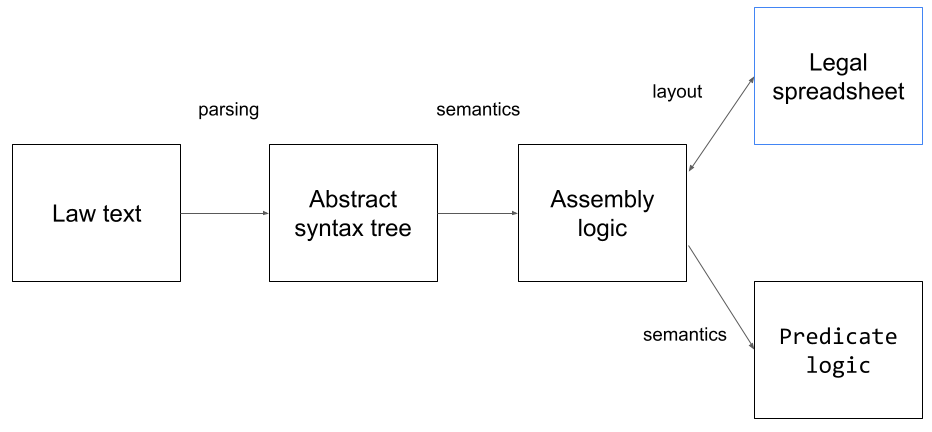
\includegraphics[width=0.8\textwidth]{pipeline.png}
\caption{The pipeline}
\label{pipeline}
\end{figure}


% , while Fig.\ref{pipeline-ex} shows a concrete example of its use on a paragraph of text.
% The second step is converting the abstract syntax trees resulting from the parser into formulas in an \textbf{assembly logic}.
% This is an intermediate representation between abstract syntax trees and normal ``back end'' logics such as predicate logic.
% It is more abstract than the syntax trees coming from the parser, but preserves more distinctions than, say, predicate logic.
% These distinctions are particularly useful when deriving visualizations of the structure, such as \textbf{spreadsheets}, two-dimensional representations that make the logical structure explicit without using logical formulas.
% These visualizations are intended to help understand the text and also to select proper interpretations of it in case of ambiguity.
% The conversion is performed in Haskell using the methodology described in \cite{ranta-2011c}.

% context-free grammar automatically derived from the text itself.
% At a later phase, we can optionally replace this with a richer kind of GF grammar.

% the structure, such as \textbf{spreadsheets}, two-dimensional representations that make the logical structure explicit without using logical formulas.
% These visualizations are intended to help understand the text and also to select proper interpretations of it in case of ambiguity.
% The conversion is performed in Haskell using the methodology described in \cite{ranta-2011c}.

\subsection{From Law Text to ASTs}
\label{sec:2.2}

GF parsers are driven by grammars, such as GF's general-purpose Resource Grammar Library (RGL, \cite{ranta-2009}).
However, the RGL is not sufficient for law texts, which contain special constructs that are essential for the logical structure, such as itemised lists and indented paragraphs.
Thus we developed a tailored grammar on top of the RGL.
We started in a data-driven, top-down manner, starting from the text itself.
To this end, we developed a semi-automatic method where the user annotates the text and a Haskell script generates GF rules the annotated text.
The rules are generated in a context-free format that GF software can process.
Figure~\ref{grammar-gen} illustrates the grammar building workflow.

\begin{figure}[h!]
 \begin{framed}
\bequ
\textbf{A line in the raw text:}
\bequ
\textit{(2) without limiting subsection (1)(a), a data breach is deemed to result in significant harm to an individual ---}
\enqu
\textbf{The line annotated with marks for terminals} (\verb6#6) \textbf{and nonterminals} (\verb6*6):
\bequ
\begin{verbatim}
*Item (2) #without #limiting #subsection *Ref (1)(a) #,
#a *CN data breach #is #deemed #to
*VP result in significant harm to an individual #-
\end{verbatim}
\enqu
\textbf{Grammar rules derived automatically by the script:}
\bequ
\begin{verbatim}
Line ::= Item "without" "limiting" "subsection" Ref ","
         "a" CN "is" "deemed" "to" VP "-" ;
Item ::= "(2)" ;
Ref  ::= "(1)(a)" ;
CN   ::= "data" "breach" ;
VP   ::= "result" "in" "significant"
         "harm" "to" "an" "individual" ;
\end{verbatim}
\enqu
\textbf{The VP rule above refined into more general rules:}
\bequ
\begin{verbatim}
VP2 ::= "result" "in" NP ;
NP  ::= "significant" "harm" "to" NP ;
NP  ::= "an" CN ;
CN  ::= "individual" ;
\end{verbatim}
\enqu
%\textbf{The same four rules converted into GF abstract syntax functions:}
%\bequ
%\begin{verbatim}
%fun VP2_result_in : VP2 ;
%fun CN_significant_harm_to_NP : NP -> CN ;
%fun NP_an_CN : CN -> NP ;
%fun CN_individual : CN ;
%\end{verbatim}
%\enqu
%\textbf{Manually merging morphological variants (with rules derived elsewhere):}
%\bequ
%\sout{\texttt{fun CN\_individuals : CN ;}} \\
%\texttt{fun CN\_individual : CN ;} {\it --- automated choice of singular vs. plural}
%\sout{\texttt{fun NP\_an\_CN : CN -> NP ;}} \\
%\texttt{fun NP\_a\_CN  : CN -> NP ;} {\it --- automated choice of `a' vs. `an'}
%\enqu
\enqu
\end{framed}
\caption{The grammar extraction process.}
\label{grammar-gen}
\end{figure}



\subsection{From ASTs to Assembly Logic}
\label{sec:assembly-logic}

Assembly logic is an intermediate representation between ASTs and standard logics.
It is designed to preserve enough syntactic structure to generate representations that humans can easily relate to the original text.
For example, it distinguishes between ordinary and reverse implications (``if A then B'' vs.\ ``B if A'') and preserves quantified noun phrases as units (e.g.\ ```any organisation'').
It is intended to be sufficient for this purpose, so that when the grammar is extended (e.g., new law texts), the assembly logic and its back-ends can be kept constant.

Figure~\ref{assembly} shows a sample of the assembly logic implemented as a Haskell datatype \texttt{Formula}.
It also shows part of an \textbf{interpretation function} \cite{ranta-2011c}, \texttt{iNP}, which converts ASTs of GF type \texttt{NP} (Noun Phrase) to assembly logic.
These functions use pattern matching over trees.
Each AST constructor may have its own pattern, such as for \verb6NP_any_CN6 in Figure~\ref{assembly}.
When the grammar is extended, new patterns can be added.
But even if this is not done, the function can take care of the new constructors by the catch-all case (\verb6_6) which treats the new expressions as atomic.
Atomic expressions can then be converted to atomic formulas or constants in logics and to single cells in spreadsheets (see Section~\ref{sec:vis:spreadsheets}).

\begin{figure}
  \begin{framed}
 \bequ
 \textbf{Some assembly logic constructors:}
 \enqu

\bequ
\begin{verbatim}
  data Cat =
    CProp | CSet | CInd | ...
  data Formula =
    Atomic Cat Atom
  | Implication Formula Formula
  | Conditional Formula Formula     -- reverse implication
  | Quantification String Formula   -- quantifier + domain
\end{verbatim}
 \enqu
 \bequ
 \textbf{Semantics of ASTs in the assembly logic:}
\enqu
\bequ
\begin{verbatim}
  iNP :: Env -> NP -> Formula
  iNP env np = case np of
    NP_any_CN cn -> Quantification "ANY" (iCN env cn)
    NP_each_CN cn -> Quantification "EACH" (iCN env cn)
    ...
    _ -> Atomic CInd (toAtom env np) -- convert to string
\end{verbatim}
 \enqu

   \end{framed}
\caption{Data structures and conversions related to the assembly logic.}
\label{assembly}
\end{figure}

\subsection{From Assembly Logic to Predicate Logic}
\label{sec:predicate-logic}

Assembly logic is first mapped into a many-sorted logic, which is then mapped into ordinary predicate logic and rendered in TPTP \cite{sutcliffe2009tptp} notation. 
We use many-sorted logic because it better supports compositional translation.
Thus quantification expressed by noun phrases (e.g.\ ``any organisation'') are compositionally interpreted as quantifiers with sorts rather than divided into unsorted quantifiers and sort predicates, whereas definite noun phrases  (e.g.\ ``that organisation'') are interpreted as Russell's iota terms (we write $\iota(A)$ instead of $(\iota x)A(x)$, leaving possible variable bindings to $A$ itself, as is customary in higher-order logic).

Both sorted quantifiers and iota terms are eliminated during the conversion from many-sorted to ordinary predicate logic.
Iota terms are eliminated in a pass that looks for non-iota terms in their context of use.
Here is a minimal example, with an existential quantifier in the antecedent and definite noun phrase referring to it in the succedent:
\bequ
        \textit{if a notification is a data breach, the notification is affected}
 \enqu
Its compositional interpretation in many-sorted logic with iota terms is
\[
(\exists x : \eop{notification})\eop{data\_breach}(x) \, \supset \, \eop{affected}(\iota(\eop{notification}))
\]
When converted to ordinary predicate logic, the existential quantifier is changed into a universal one with a wide scope of implication, and the iota term is interpreted as the bound variable:
\begin{verbatim}
  ![X]:(notification(X) => data_breach(X) => affected(X))
\end{verbatim}
%Figure~\ref{donkey} shows an example from real law text, with an inverted conditional.
%Note that the logic output still has unanalysed parts treated as atomic predicates.
%
%\begin{figure}
%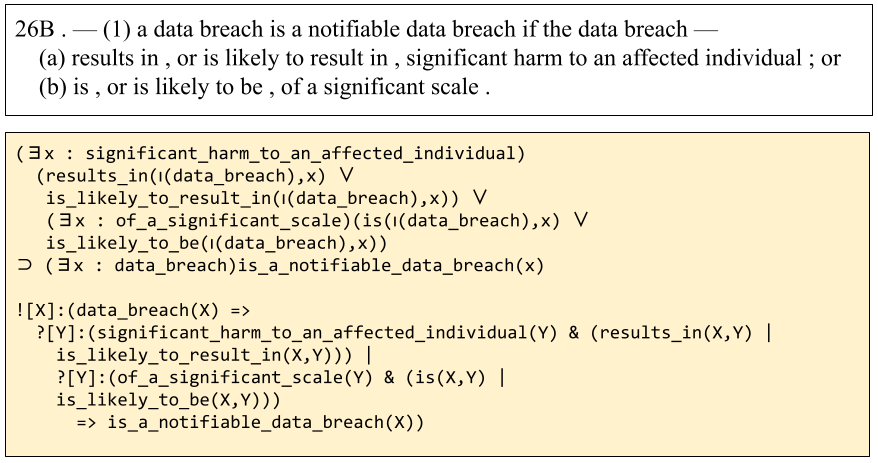
\includegraphics[width=0.96\textwidth]{anaphora.png}
%\caption{An inverted conditional in the actual law text interpreetd in the two logics.}
%\label{donkey}
%\end{figure}

\subsection{From Assembly Logic to Spreadsheets}
\label{sec:vis:spreadsheets}

The AST can also be automatically visualised in a spreadsheet (see Figure \ref{pipeline-ex}) displaying the formula trees in a structured format (like in \cite{mochales_study_2008}). The spreadsheet format, which serves as the input to a low-code programming platform, is currently under development and will be more fully described in future work.

\section{Formalizing the Personal Data Protection Act}
\label{sec:pdpa}

We illustrate our pipeline using Part 6A of the PDPA. Like the EU's \textit{General Data Protection Regulation} (GDPR), the PDPA is Singapore's primary data protection statute and prescribes obligations surrounding the collection, use, disclosure, and deletion of personal data. Part 6A stipulates when and how organisations are expected to notify regulators of data breaches. We use the PDPA as a case study for three reasons. First, this was a practical suggestion from Singapore's Personal Data Protection Commission (who hypothesised that formalizing the PDPA would help them better manage legislative change).
Second, while the PDPA has not been examined in AI \& Law literature, its subject matter connects it to prior work on the GDPR \cite{palmirani_modelling_2018,palmirani_legal_2018,hickey_gdpr_2021}.
Third, Part 6A is complex enough to demonstrate the utility of a computational law approach in general and our pipeline in particular. Indeed, modelling these rules allowed us to detect a race condition in the PDPA: an organisation which informed both the Commission and the affected individuals of a data breach, as s~26D PDPA generally requires, might inadvertently violate s~26D(6) which provides that organisations should \textit{not} inform affected individuals if the Commission so directs.

The text in Part 6A of the PDPA consists of 47 lines, 1053 tokens, 228 unique tokens.
Figure \ref{pipeline-ex} below illustrates the pipeline as applied to one paragraph.

\begin{figure}
    \bequ
    \textbf{A paragraph in the raw text:}
    \enqu
    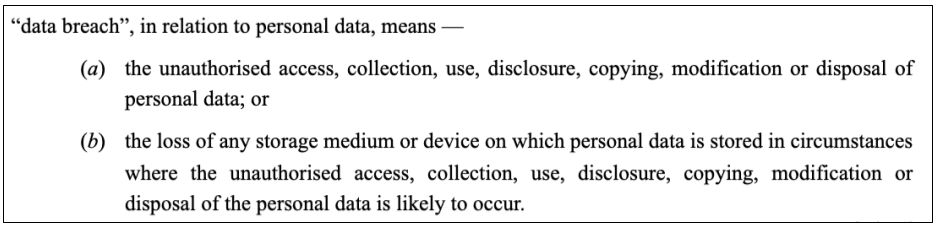
\includegraphics[width=0.7\textwidth]{text.png}

    \bequ
    \textbf{AST of line (a) and spreadsheet visualization of the paragraph}
    \enqu
    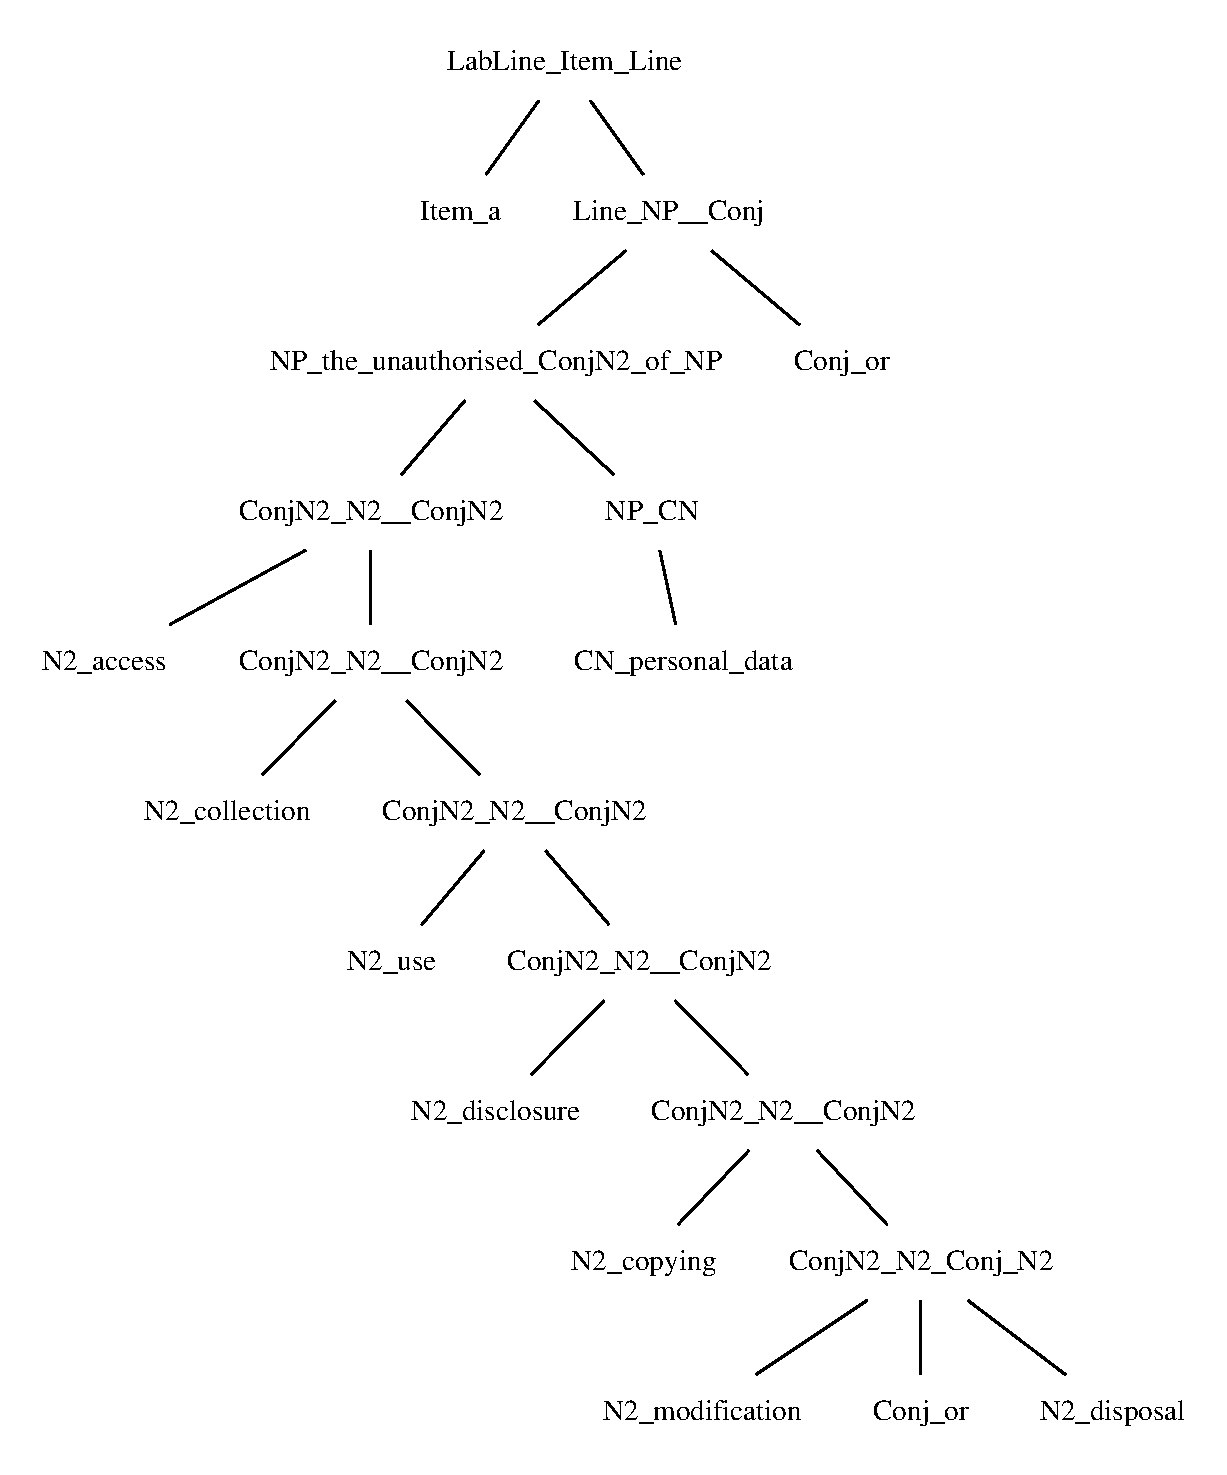
\includegraphics[width=0.36\textwidth]{tree.eps} 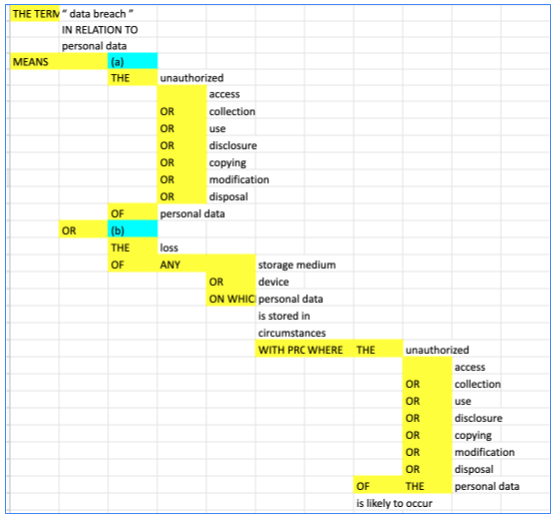
\includegraphics[width=0.48\textwidth]{assembly.png}
      \bequ
      \textbf{Logical formula in TPTP notation:}
      \enqu
    \bequ
    \tiny
    \begin{verbatim}
  ![X]:(data_breach(X) & ?[Y]:(personal_data(Y) & IN_RELATION_TO(X,Y)) <=>
  (personal_data(X) & ?[Y]:((access(Y,X) | collection(Y,X) | use(Y,X) | disclosure(Y,X) | 
  copying(Y,X) | modification(Y,X) | disposal(Y,X)) & unauthorized(Y))) | (((storage_medium(X) |   
  device(X)) & (personal_data(X) & ?[Y]:((circumstances(Y) & (((unauthorized(Y) & (access(Y) |
  collection(Y) | use(Y) | disclosure(Y) | copying(Y) | modification(Y) | disposal(Y))) &
  is_likely_to_occur(Y))) & is_stored_in(X,Y)))) & loss(X))))
    \end{verbatim}
    \enqu
\caption{An example through the pipeline: text, abstract syntax tree (of the second line), spreadsheet, and formula in TPTP notation.}
\label{pipeline-ex}
\end{figure}

\section{Conclusion}
\label{sec:discussion}
%%Converting law to logic is a known hard problem.
In this paper, we developed a pipeline that parses legal text into ASTs using the GF grammar formalism, an intermediate assembly logic, and finally predicate logic. %%That such a pipeline was successfully developed demonstrates the promise of this approach.
While manual effort was still required at various stages, the process was less tedious than a completely manual one.
More importantly, some pipeline steps can work out of the box when the input scope is extended.
The main things to be added are text annotations for extending the grammar, and the conversion of the new grammar rules to the assembly logic.
These steps light-weight enough to make the system feasible to apply to new texts.
Further, since GF's mapping between ASTs and natural language is fully reversible, the pipeline can be extended to support natural language generation. Once parsed into GF trees, the source text can be converted into novel forms: declarative sentences can become questions, negations, hypotheticals, etc. 

The work is a proof of concept and has a some limitations.
The most important one is that we have not verified the accuracy of our PDPA formalisation.
A proper eveluation would reguire gold standards developed by human legal and technical experts and vetted by the relevant regulatory body.
Thus the legal language barrier is far from solved, but we hope to have taken one more step towards realising that vision.

% Future papers will link this pipeline with other work at CCLAW: on the spreadsheet syntax, the logical semantics, and the grammar of smaller units.

% \todoj{feel free to condense this paragraph into as few words as you like!}

% The GF trees are so far used to parse text. However, the manually refined rules (merging singular and plural, `a` vs. `an` from Figure~\ref{grammar-gen}) carry all potential for generating natural language output: the more general and powerful grammar knows when to \textit{output} a singular or plural form, guaranteeing a grammatically correct text. Parts of the parsed source text can be modified into novel forms for different communicative needs: they can become questions, negations, hypotheticals etc.

% It also remains to see how much of the line and paragraph structures is already included in the grammar based on the sample, but the variation there can be expected to be numerically smaller.

\bibliographystyle{vancouver}
\bibliography{complaw-bib}

\end{document}
